\documentclass[12pt, fleqn]{article}
\usepackage{../../../template/template}

%сам документ
\begin{document}
\begin{center}
  \huge Лекции по алгебре, 3 сем
  
  \Large (преподаватель Демченко О. В.)
  
  \large Записали Костин П.А., Щукин И.В.
\end{center}

Данный документ неидеальный, прошу сообщать о найденных недочетах в \href{https://vk.com/drab_existence_a}{вконтакте}
\tableofcontents
\newpage

%билеты
\section{Теория групп}
\subsection{3.09.2019}

\begin{definition}
    G - мн-во, $*:G*G \Ra G,\ (g_1, g_2) \Ra (g_1*g_2)\ (g_1g_2)$
    \begin{enumerate}                               
    	\item $(g_1g_2)g_3 = g_1(g_2g_3) \q \forall g_1, g_2, g_3 \in G$
    	\item $\exists e \in G : e g = g e = g \q \forall g \in G$
    	\item $\forall g \in G \q \exists \widetilde{g} \in G : g\widetilde{g} = g \widetilde{g} = e$
    	\item $g_1g_2 = g_2g_1 \q \forall g_1, g_2 \in G$ - тогда это абелева группа
	\end{enumerate} 
\end{definition}

\begin{example}
    \begin{enumerate}  
        \item $(\Z,+)$ - группа
        \item $(\Z, \bullet)$ - не группа
        \item $(R, +)$ - группа кольца
        \item $(R^*, \bullet)$
        \item Группа самосовмещения $D_n$, например $D_4$ - квадрат, композиция - группа, $|D_n|=2n$
        \item $GL_n(K) = \{A \in M_n(K) : |A| \neq 0\}$, умножение - группа
        \item $\Z n \Z$ - частный случай п.3,4
    \end{enumerate} 
\end{example}

\begin{properties}[групп]
    \begin{enumerate}  
        \item e - единственный, $e,e'$ - нейтральные: $e=e e'=e'$
        \item $\widetilde{g}$ - единственный
        
        Пусть $\widetilde{g},\hat{g}$ - обратные, тогда $\widetilde{g}g = g\widetilde{g} = e = \hat{g}g = g\hat{g}$
        
        $\hat{g}=e \hat{g}=(\widetilde{g}g)\hat{g}=\widetilde{g}(g\hat{g})=\widetilde{g}e=\widetilde{g}$
        \item $(a b)^{-1}=b^{-1}a^{-1}$
        
        Это верно, если $(ab)(b^{-1}a^{-1})=(b^{-1}a^{-1})(ab)=e$, докажем первое:
        
        $(ab)(b^{-1}a^{-1})=((ab)b^{-1})a^{-1}=(a(b b^{-1}))a^{-1}=(a e)a^{-1}=a a^{-1}=e$
        \item $(g^{-1})^{-1}=g$
    \end{enumerate} 
\end{properties}

\begin{definition}
    $g \in G \q n \in \Z$, тогда $g=
\left[ 
  \begin{gathered} 
    \overbrace{g...g}^n, \q n>0\\
    e, \q n=0\\ 
    \underbrace{g^{-1}...g^{-1}}_n, \q n<0
  \end{gathered} 
\right.$
\end{definition}

\begin{properties}[степени]
    \begin{enumerate}                               
    	\item $g^{n+m}=g^n g^m$
    	\item $(g^n)^m=g^{n m}$
	\end{enumerate} 
\end{properties}

\begin{definition}
    $g \in G$, $n \in N$ - порядок g $(\ord g = n)$, если:
    \begin{enumerate}                               
    	\item $g^n=e$
    	\item $g^m=e$ $\Ra$ $m \geqslant n$
	\end{enumerate} 
\end{definition}

\begin{example}
    \begin{enumerate}                               
    	\item $D_4$ $\ord$(поворот $90\degree) =4$
    	
    	$D_4$ $\ord$(поворот $180\degree) =2$
    	\item $(\Z /6 \Z, +)$ $\ord(\overline{1})=6$
    	
    	$\ord(\overline{2})=3$
	\end{enumerate} 
\end{example}

\begin{utv}
    $g^m=e \q \ord(g)=n$ $\Ra$ $m \devides n$ (n>0)
\end{utv}
\begin{proof}
    $m=n q+r$, $0 \leqslant r < n$
    \\
    $e=g^m=g^{n q + r}=(g^n)^q g^r=g^r$ $\Ra$ $r=0$
\end{proof}

\begin{definition}
    $H \subset G$ называется подгруппой G (H < G) (и сама является группой), если:
    \begin{enumerate}                               
    	\item $g_1,g_2 \in H \Ra g_1 g_2 \in H$
    	\item $e \in H$
    	\item $g \in H \Ra g^{-1} \in H$
	\end{enumerate} 
\end{definition}

\begin{example}
    \begin{enumerate}                               
    	\item $n\Z < \Z$
    	\item $D_4$
    	\item $SL_n(K)=\{A \in M_n(K): \q |A|=1\}$, $SL_n(K)<GL_n(K)$
	\end{enumerate} 
\end{example}

\begin{tabular} {c|c}
	Мультипликативная запись & Аддитивная запись\\ \hline 
	$g_1 g_2$ & $g_1 + g_2$\\
	$e$ & $0$\\
	$g^{-1}$ & $-g$\\
    $g^n$ & $n g$ 
\end{tabular}

\begin{definition}
    $H<G$, $g_1,g_2 \in G$, тогда $g_1 \sim g_2$, если:
    \begin{enumerate}                               
    	\item $g_1=g_2 h$, $h \in H$ (левое)
    	\item $g_2=h g_1$, $h \in H$ (правое)
	\end{enumerate} 
\end{definition}

\begin{proof}[эквивалентности]
    \begin{enumerate}                               
    	\item (симметричность) $g_1=g_2 h \overset{*h^{-1}}{\Ra} g_2 = g_1 h^{-1}$
    	\item (рефлексивность) $g=g e$
    	\item (транзитивность) $g_1=g_2 h$, $g_2 = g_3 h$ $\Ra$ $g_1=g_3(h_2 h_1)$, где $h_2 h_1 \in H$
	\end{enumerate} 
\end{proof}

\begin{definition}
    $[a] = \{b:a ~ b\}$ классы эквивалентности
\end{definition}

\begin{definition}
    $[g] = g H = \{g h, h \in H \}$ (левый класс смежности) 
    \\
    $g h \sim g \Ra g h \in [g]$
    \\
    $g_1 \in [g] \Ra g_1 \sim g \Ra g_1 = g h$
\end{definition}

\begin{utv}
    $[e]=H$
    \\
    Установим биекцию: 
    \\
    $[g]=g h \leftarrow H$
    \\
    $g h \leftarrow h$
    \\
    Очевидно, сюръекция, почему инъекция? 
    \\
    $g h_1 = g h_2 \overset{*g^{-1}}{\Ra} h_1 = h$
\end{utv}

\begin{theorem}[Лагранжа]
$H < G$, $|G| < \infty$, тогда $|G| \devides |H|$ (уже доказали!)
\end{theorem}
\subsection{10.09.2019}

\begin{consequence}
    G - кон. группа, $a \in G$, $\ord a = m$, $H=\{a^n:n \in \Z\}$, тогда $|H|=m$\\
\end{consequence}

\begin{proof}
    $\{a^0=e,a_1,...,a^{m-1}\}$ - подмножество H\\
    Докажем, что все остальные элементы тоже здесь есть\\
    $n \in \Z \Ra n=m q+r$, $0 \leqslantr \leqslant m-1$\\
    $a^n=a^{m q+r}=(a^m)^q a^r=a^r$\\
    $a^k=a^l$, $0 \leqslant k \leqslant l \leqslant m-1$, умножим на $a^{-k}$\\
    $e=a^{l-k}$ $o \leqslant l-k \leqslant m-1$ m - наименьшее $\N$ такое что $a^m=e$\\
    $l-k=0 \Ra l=k$\\
    Докажем, что $|H|=m$\\
    $\Ra |G| \devides m=\ord a$, т.о. в группе порядок эл-та - делитель порядка группы
\end{proof}

Напоминание 

\begin{consequence}[теорема Эйлера]
    $n,a \in \N$, $(a,n)=1$, тогда $a^{\varphi(n)} \equiv 1 (mod n)$
\end{consequence}

\begin{proof}
    Рассмотрим $G=(\Z / n \Z)*$ $|G|=\varphi(n)$\\
    $\overline{a} \in G$, $\ord \overline{a}=k$\\
    $\varphi(n) \devides k \Ra \varphi(n) = kl$\\
    $\overline{a}=\overline{1}$\\
    $\overline{a}^{\varphi(n)}=\overline{1}$
\end{proof}

\begin{definition}
    G - циклическая группа, если $\e g \in G: \forall g' \in G: \e k \in \Z: g'=g^k$\\
    Такой g называется образующим
\end{definition}

\begin{example}
    $\Z$ (образующий - единица и минус единица)
\end{example}

\begin{remark}
    Любая циклическая группа - коммунитативна
\end{remark}

\begin{proof}
    $g' g'' = g'' g' = g^k g^l = g^l g^k$
\end{proof}
\\
Пусть G,H - группы, рассмотрим $G \times H = \{(g,h): g\in G, h\in H\}$\\
Введем операцию $(g,h)*(g',h')\overset{def}{=}(g*_G g', h*_H h')$\\
Докажем, что это группа.\\
Доказательство ассоциативности:
\[((g,h)(g',h'))(g'',h'') \overset{?}{=} (g,h)((g',h')(g'',h'')\]
\[(g g',h h')(g'',h'') \overset{?}{=} (g,h)(g' g'', h' h'')\]
\[((g g')g'',(h h')h'') \overset{?}{=} (g(g',g''),h(h'h'') \text{ - очевидно}\]
Нейтральный элемент:

Рассмотрим $\Z /2 \Z \times \Z /2 \Z = \{(\overline{0},\overline{0}),(\overline{0},\overline{1}),(\overline{1},\overline{0}),(\overline{1},\overline{1})\}$

\begin{utv}
    Конечная группа порядка n является циклической тогда и только тогда, когда она содержит элемент порядка n ($|G|=n$, G - циклическая $\equiv$ $\e g \in G: \ord g = n$)
\end{utv}
Рассмотрим $\Z /2 \Z \times \Z /3 \Z$ - циклическая\\
$((\overline{1},\overline{1}), (\overline{0}, \overline{2}), (\overline{1}, \overline{0}), (\overline{0}, \overline{1}), (\overline{1},\overline{2}))$\\
Рассмотрим $\Z /2 \Z \times \Z /4 \Z$ - не циклическая

\begin{definition}
    $\varphi: G \ra H$ - биекция и $\varphi(g_1,g_2)=\varphi(g_1) \varphi(g_2)\q \forall g_1,g_2 \in G$, тогда $\varphi$ - изоморфизм 
\end{definition}

\begin{instance}
    \begin{enumerate}
        \item $D_3 \ra S_3$
        \item $U_n=\{z\in \CC: z^n=1\} \la \Z / n \Z$\\
        ($\frac{2\pi a}{n}+i \sin \frac{2\pi a}{n} = \varphi \overline{a} \mapsfrom \overline{a}$)\\
        $\overline{a}=\overline{b} \ra \varphi(\overline{a})=\varphi(\overline{b})$\\
        $\varphi(\overline{a}+\overline{b}) \overset{?}{=} \varphi(\overline{a})\varphi(\overline{b})$\\
        $\cos \frac{2\pi(a+b)}{n}+i \sin \frac{2\pi(a+b)}{n}=(\cos\frac{2\pi a}{n} + i \sin \frac{2\pi a}{n}) $
    \end{enumerate}
\end{instance}

\begin{definition}
    Две группы называются изоморфными, если между ними существует изоморфизм
\end{definition}

\begin{utv}
    Изоморфизм - отношение эквивалентности
\end{utv}

\begin{proof} \ \\
    т.к. композиция изоморфизмов - изоморфизм $G \overset{e}{\ra} H \overset{\psi}{\ra} H$\\
    $(\psi \circ \varphi)(g_1 g_2)= \psi(\varphi(g_1 g_2)=\psi(\varphi(g_1) \varphi(g_2))=\psi(\varphi(g_1)) \psi(\varphi(g_2)) = (\psi \circ \varphi)(g_1) \circ (\psi \circ \varphi)(g_2)$\\
    Рефлексивность - тождественное отображение - изоморфизм\\
    Транзитивность: $G \underset{\varphi}{\ra} H$, $H \underset{\varphi^{-1}}{\ra} G$
\end{proof}

\begin{theorem}
    G - циклическая группа\\
    1) $|G|=n \Ra G \cong \Z / n \Z$\\
    2) $|G|=\infty \Ra G \cong \Z$
\end{theorem}

\begin{proof}\\
    1) g - обр. G, значит $G=\{e,g,g^2,...,g^{n-1}\}$ (среди них нет одинаковых), построим изоморфизм в $\Z / n \Z$: $\varphi(g^k)=\overline{k}$\\
    Проверим, что $\varphi(g^k g^l)= \varphi(g^k)+\varphi(g^l)=\overline{k}+\overline{l}$\\
    Левая часть: $\varphi(g^{k+l}=\overline{(k+l) \mod n} = \overline{k}+\overline{l}$\\
    2) $G=\{...,g^{-1},e,g,g^2,...\}$ (тоже нет совпадающих элементов, иначе $g^k=g^l$, при $k>l$, тогда $g^{k-l}=e$, но тогда конечное число элементов, потому что оно зацикливается через каждые $k-l$ элементов), построим отображение в $\Z$.\\
    $\varphi(g^n)=n$ -, очевидно, биекция. И нужно доказать, что $\varphi(g^n g^k)=\varphi(g^n)-\varphi(g^k)=n+k$
\end{proof}

\subsection{17.09.2019}
\begin{utv}
    $|G|=p$, p - простое $\Ra$ $G \cong \Z /p \Z$
\end{utv}

\begin{proof}
    $g \in G$, $g \neq e$, $\ord g=p$
    
    $\Ra G=\{e=g^0,g,...,g^{p-1}\}$
\end{proof}

\begin{utv}
    $H,G$ - группы, $\varphi: G \ra H$ - изоморфизм $\Ra$ $n=\ord g=\ord \varphi(g)$
\end{utv}

\begin{proof}
    Пусть $g^n=e,\ \varphi(g^n)=\varphi(e)\os{?}{=}e$
    \[\varphi(e)^2=\varphi(e^2)=\varphi(e)\]
    Теперь докажем, что меньшего нет
    \[\varphi(g)^m = e,\ m \in \N \os{?}{\Ra} m \geqslant n\]
	\[\varphi(g^m) = \varphi(g)^m = e = \varphi(e) \q \Ra g^m = e \Ra m \geq n\]
\end{proof}

\begin{definition}
    $H<G$, тогда H - нормльная подгруппа, если $\forall h \in H, g \in G \Ra g^{-1}h g \in H$ - сопряжение элемента h с помощью элемента g, обозначается: $H \triangleleft G$
\end{definition}

\begin{remark}
    Элементы подгруппы при сопряжении переходят в элементы подгруппы
\end{remark}

\begin{remark}
    Подгруппа любой коммунитативной группы нормальна
\end{remark}

\begin{example}
    $D_3$ - 6 элементов, 3 поворота и 3 симметрии
    
    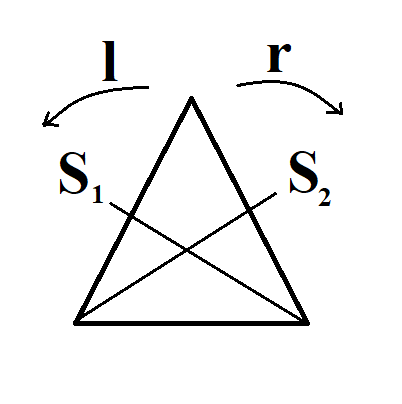
\includegraphics[scale=0.3]{pics/triangle_d_3.png}
    
    $\{e,l,r\}$ - нормальная
    
    $\{e, s_1\}$ - не нормальная
\end{example}

\begin{utv}
    $H \triangleleft G$ $\lra$ разбиение на Л и П кдассы смежности по H совпадают
    \[\forall g \q gH = Hg\]
\end{utv}

\begin{proof}
    Берем произвольный элемент из левого и правого и докажем, что совпадают. Берем слева:
    \[h \in H \q g h \in g H\]
    \[g h = \underbrace{(g^{-1})^{-1} h g^{-1}}_{\in H} g = h_1 g\]
    Теперь справа:
    \[g \in G,\q h \in H,\q g^{-1}h g=h_1\]
    \[h g \in H g = g H \Ra g h_1, h_1 \in H\]
\end{proof}

\begin{definition}
    $H \triangleleft G$
    $g_1 H * g_2 H \eqdef g_1 g_2 H$
\end{definition}

\begin{proof}[коррекнтности]
    Хотим проверить, что 
    \[\w{g}_1 H = g_1 H,\q \w{g}_2 H = g_2 H \os{?}{\Ra} \w{g_1}\w{g_2}H = g_1 g_2 H\]
    Аналогично прошлому доказательству 
    \[g_2^{-1}h_1 g_2 = h_3 \in H \]
    \[\widetilde{g_1}\widetilde{g_2}h = g_1 h_1 g_2 h_2 h = g_1 g_2 (\us{= h_3}{g_2^{-1}h_1 g_2})h_2 h\]
    \[\widetilde{g_1}H = g_1 H \Ra \widetilde{g}_1 = g_1 h_1\]
    \[\widetilde{g_2}H = g_2 H \Ra \widetilde{g_2} = g_2 h_2\]
    Не использовали условие $g_2^{-1} h_1 g_2 = h_3 \in H$
    \[\w{g_1} \w{g_2} H = g_1 h_1 g_2 h_2 h = g_1 g_2 \us{=h_3}{(g_2^{-1} h_1 g_2) }h_2 h\]
    Осталось доказать, что получается группа
    \[\text{1) Нейтральный элемент}\q e H=H,\q e H * g H = (e g) H = g H\]
    \[\text{2) Ассоциативность}\q (g_1 H+g_2 H)*g_3 H \os{?}{=} g_1 H*(g_2 H * g_3 H)\]
    \[(g_1 g_2)H * g_3 H = (g_1 g_2)g_3 H\]
    \[3)\q gH * g^{-1}H = (g g^{-1})H = eH \]
\end{proof}

\begin{What}
    \[G/H\]
    \[\text{Была эквивалентность: }a \sim b \rla a - b \ \vdots \ h\]
    \[G = \Z\]
    \[H=h \Z,\q g_1 g_2^{-1} \in H\text{ - мульт. запись },\q g_1-g_2 \in n \Z\text{ - адд. запись}\]
    \[[a] + [b] = [a + b]\]
    Аддитивная группа кольца класса вычетов - это то же самое, что фактор группа группы $\Z$ по подгруппе $n\Z$
\end{What}

\begin{example}
    Как в произвольной группе найти подгруппу?
    
    $[g,h]=g h g^{-1} h^{-1}$, $g,h \in G$ - коммутатор элементов $h,g \in G$
    
    Коммутант - множество проззведений всех возможных коммунтаторов
    
    Обозначается $K(G)=\{[g_1,h_1]...[g_n,h_n],\ g_1,h_1 \in G\}$
\end{example}

\begin{proof}[коммутант - подгруппа]
    $K(G)<G$
    
    Нейтральный элемент: $[e,e]=e$
    
    Обратный элемент? $[g_1,h_1]...[g_n,h_n]$
    
    Как его найти? $[g,h^{-1}]^{-1}=(g h g^{-1} h^{-1})^{-1}=h g h^{-1} g^{-1}=[h,g]$
    
    $([g_1,h_1]...[g_n,h_n])^{-1}=[g_1,h_1]...[g_n,h_n]$
    
    Значит это подгруппа
    
    Нормальная ли? $g^{-1}[g_1,h_1]...[g_n,h_n]g$
    
    $g^{-1} [g_1,h_1] g (g^{-1} [g_2,h_2]g)...(g^{-1} [g_n, h_n] g)$
    
    Нужно доказать, что сопряжение коммунтатора лежит в коммутанте
    
    $g^{-1} g_1 h_1 g_1^{-1} h_1^{-1} g = \underbrace{g^{-1} g_1 h_1 g_1^{-1} h_1^{-1}}_{=[g^{-1 g_1,h_1}]} \underbrace{h_1 g^{-1} h_1^{-1} g}_{=[h_1,g^{-1}]}$
\end{proof}

\begin{utv}
    Фактор-группа ($G / K(G)$) по коммутанту - коммунитативна
\end{utv}

\begin{Proof}
    \[g_1, g_2 \in G \q\q g_1 K(G) g_2 K(G) \os{?}{=} g_2 K(G) g_1 K(G)\]
	\[g_1 g_2 K (G) = g_1 g_2 K(G) \q\q g_2 K(G) g_1 K(G) = g_2 g_1 K(G)\]
	\[[g_1, g_2] = g_1 g_2 (g_2 g_1)^{-1} \in K(G) \]
\end{Proof}

\begin{Utv}
    \[\Z_n \times \Z_m \simeq \Z_{mn} \text{, если } (m, n) = 1 \]
\end{Utv}

\begin{proof}
    Нужно построить изоморфизм $[a]_{m n} \mapsto ([a]_n,[a]_m)$
    
    $[a]_{m n} = [a']_{m n} \Ra [a]_n = [a']_n$, $[a]_m=[a']_m$
    
    Теперь нужно проверить биекцию
    
    Сюръекция: $\forall b,c \in \Z$ $\e x \in \Z: \begin{cases}[x]_n=[b]_n\\ [x]_m=[c]_m \end{cases}$, по КТО всё хорошо
    
    Инъективность: {\[ \begin{align}
			&[a]_n = [b]_n\\
			&[a]_m = [b]_m
	\end{align} \Ra [a]_{m n} = [b]_{m n}\]} %конструкция Ильи, а есть без ошибок?
    
    На языке сравнений: {\[\begin{align}
		&a \equiv b(n)\\
		&a \equiv b(m)
	\end{align} \Ra a \equiv b (m n)\]}
    
    На самом деле достаточно было проверить одно
\end{proof}

\begin{Definition}
		\[\varphi : G \to H \text{ - гомоморфизм, если } \varphi(g_1 g_2) = \varphi(g_1) \varphi(g_2)\]
		\[\text{изоморфизм = гомоморфизм + биективность}\]
		\[\varphi \in \text{Hom}(G, H) \text{ - множество гомоморфизмов}\]
\end{Definition}

\begin{Examples}
	\[1)\q \CC^* \to \R^*\]
	\[z \to |z|\]
	\[2)\q GL_n(K) \to K^*\]
	\[A \to \det A\]
	\[3)\q S_n \to  \{\pm 1\}\]
	\[\sigma \to \left\{ \begin{align}
			&+1,& &\text{ если } \sigma \text{ - четн.}\\
			&-1,& &\text{ если } \sigma \text{ - неч.}
	\end{align}\]
	\[4)\q a \in G \q G \to G\]
	\[g \to a^{-1}g a\]
	\[(a^{-1}g a)(a^{-1}g_1a) = a^{-1}g_1 g a \]
\end{Examples}
\end{document}